\chapter{Implementación}

\section{Modelos}

\begin{figure}[!ht]
    \centering
    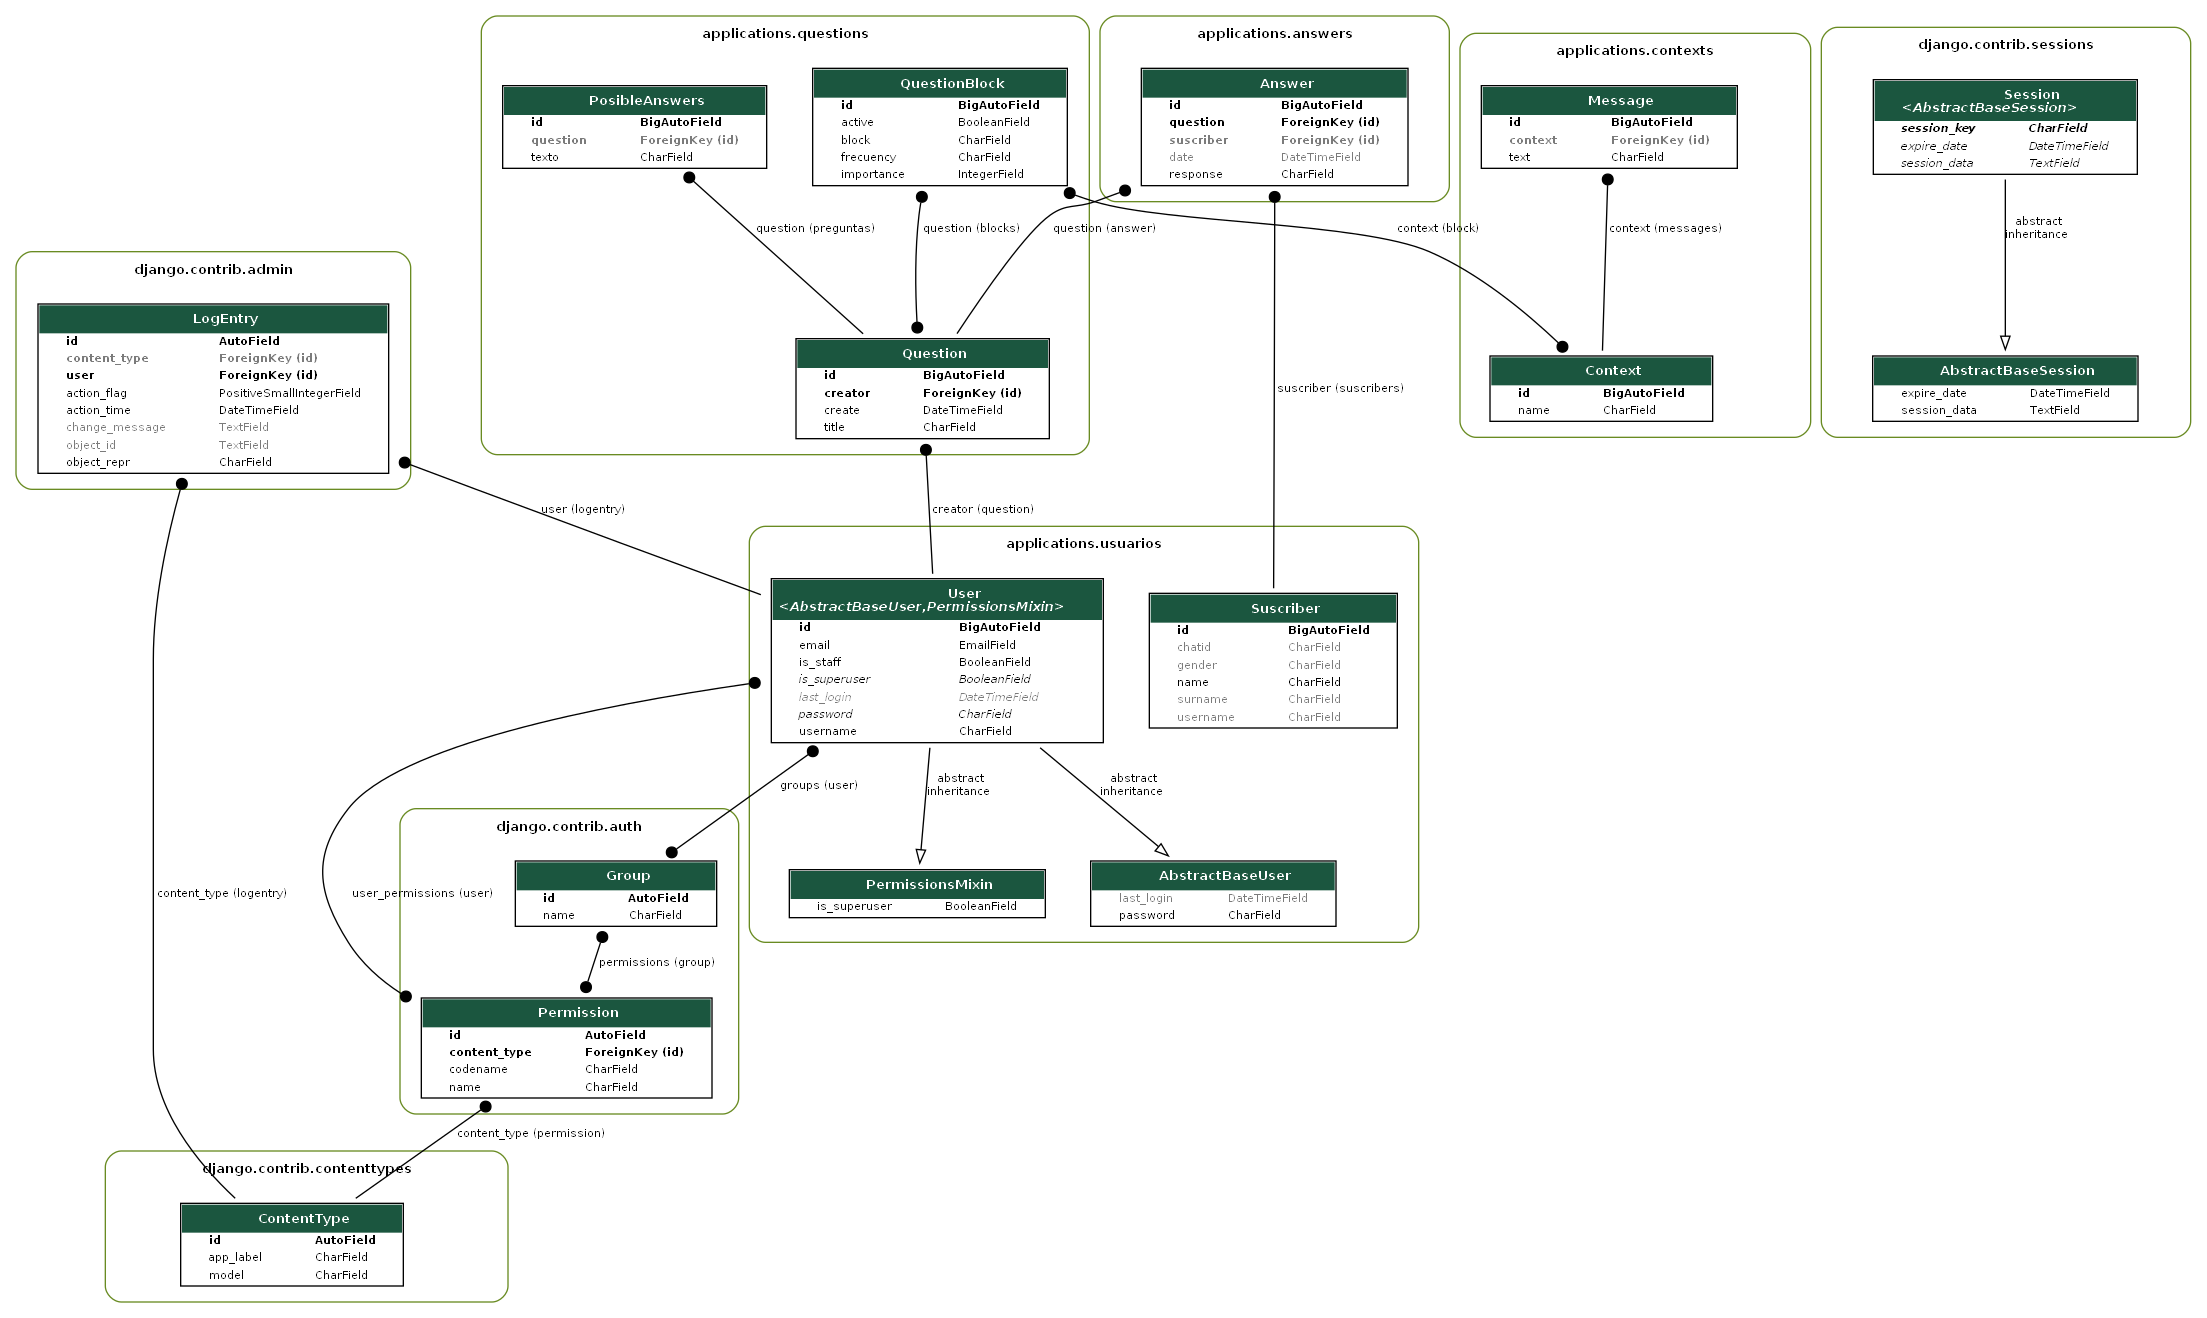
\includegraphics[width=1\textwidth, height=11cm]{imagenes/myapp_models.png}
    \caption{ Diagrama de clases }
    \label{fig:diagrama}
\end{figure}\vspace{1cm}


En la \textit{\hyperref[fig:diagrama]{Figura 5.1}} se ve el diagrama de clases que muestra las relaciones entre los modelos creados en el sistema. Siguiendo el modelo de la ORM de Django \textit{(\cite{djangoorm})}, este nos permite interactuar con bases de datos relacionales de una manera más orientada a objetos. Esta base de datos consta de cinco modelos principales:

\begin{itemize}
\item \textbf{Peguntas}: Contiene la información de todas las preguntas almacenadas. Esta se divide en dos: Pregunta y Posibles respuestas. Dentro de la primera especificaría el título de la pregunta junto con otros campos como la fecha o usuario de creación y la segunda contiene las respuestas a esa pregunta. 
\item \textbf{Bloques de Preguntas}: Las preguntas se estructuran en bloques. Cada bloque puede tener las preguntas que desee, junto a otros atributos para que permiten su planificación. Los bloques también tienen asociado un preámbulo. 
\item \textbf{Preámbulos}: Dentro de los preámbulos se guardan los mensajes a mostrar por el bot cuando se hable de un tema concreto. Si un bloque tiene asociado un preámbulo, en el momento que se realice el cuestionario asociado a ese bloque de preguntas el bot mostrará cualquiera de los mensajes de ese preámbulo de forma aleatoria. De esta forma nos aseguramos la interactividad y que la experiencia sea diferente para cada usuario.
\item \textbf{Usuarios}: Guarda los agentes registrados en nuestro sistema. Se divide en dos tipos: los administradores que tienen acceso al panel de control y los usuarios comúnes que son los que interactúan con el bot.
\item \textbf{Respuestas}: Contiene las respuestas de los usuarios a las preguntas. Solo se almacenan las respuestas posibles de cada pregunta para así confirmar que la información sea correcta.
\end{itemize}

\section{Aplicación Web}

La aplicación web se ha creado con el objetivo de proporcionar una interfaz atractiva y manejable usada como panel de administración de forma que podamos interactuar con los cuestionarios, respuestas e información mostrada en el bot. Esta solución garantiza la integridad y el almacenamiento seguro de los datos almacenados en una base de datos centralizada. 

La aplicación web funciona como intermediario entre el usuario y el bot. Esta se encarga de la creación de cuestionarios, del procesamiento y visualización de las repuestas de manera organizada, lo que facilita su posterior análisis. Nace como solución a satisfacer la importancia de la automatización y agilidad en la recopilación de datos, logrando un enfoque integral para la administración y respuestas de usuarios.

El chatbot se ha pensado para ser utilizado por los usuarios. Sin embargo, la aplicación solo podrá ser usada por el administrador o las personas autorizadas para su uso. En este capítulo se explican los pasos seguidos para su desarrollo.º

\subsection{Patrón MVT}

Django es un framework basado en el modelo  MVC (Model-View-Controller). MVC es un patrón arquitectónico que separa una aplicación en tres componentes lógicos principales: el modelo, la vista y el controlador. Cada uno de estos componentes está diseñado para manejar aspectos de desarrollo específicos de una aplicación. Además, MVC es uno de los marcos de desarrollo web estándar de la industria más utilizados para crear proyectos escalables y extensibles.

Django implementa este patrón MVC de una manera peculiar y con algunas variaciones que ellos llaman MTV, que viene siendo la de Model, Template, View \textit{(\cite{djangomvt})}.

\begin{itemize}

\item M significa "Model" (Modelo), la capa de acceso a la base de datos. Esta capa contiene toda la información sobre los datos: cómo acceder a estos, cómo validarlos, cuál es el comportamiento que tiene, y las relaciones entre los datos.

\item T significa "Template" (Plantilla), la capa de presentación. Esta capa contiene las decisiones relacionadas a la presentación: como algunas cosas son mostradas sobre una página web u otro tipo de documento.

\item V significa "View" (Vista), la capa de la lógica de negocios. Esta capa contiene la lógica que accede al modelo y la delega a la plantilla apropiada: puedes pensar en esto como un puente entre el modelos y las plantillas.

\end{itemize}

Esta es la lógica seguida para el desarrollo. Si nos adentramos en el codigo, vemos que existe una carpeta llamada \textit{'applications'} que contiene varias subcarpetas y en la que cada una es una tabla diferente en la base de datos. Dentro de estas subcarpetas es donde estan creadas las operaciones relacionadas con los modelos y las vistas. En un nivel superior encontramos la carperta \textit{'templates'}, que incluye las plantillas que dan funcionalidad a estas vistas, tambien separadas por modelos. Y por último dentro de la carpeta \textit{'static'} se encuentran los archivos que dan apariencia a estas plantillas.


\subsection{Login}


\begin{figure}[!ht]
    \centering
    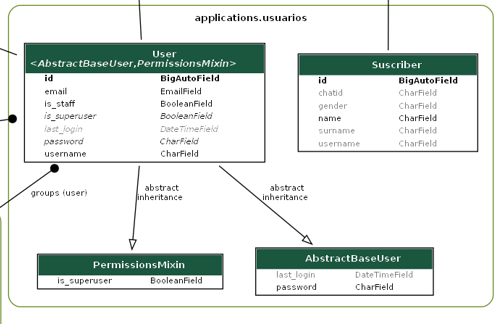
\includegraphics[width=0.8\textwidth, height=5cm]{imagenes/usuarios.png}
    \caption{ Diagrama tabla usuarios }
    \label{fig:usuarios}
\end{figure}

Existen 2 tipos de usuarios en el sistema como vemos en la \textit{\hyperref[fig:usuarios]{Figura 5.2}}

El primer usuario, identificado como \textit{User} que actua como administrador, y es el que cuenta con  todos los privilegios para poder acceder y modificar las tablas de la base de datos además de poder acceder al sistema. Y el segundo tipo \textit{Suscriber} que son los usuarios registrados por el bot sin ningún tipo de autoridad. 

En Django, las operaciones asociadas a los usuarios se manejan a través del sistema de autenticación que tiene incorporado. Permite manejar cuentas de usuario, grupos, permisos, inicios y cierres de sesión, reestablecimiento de contraseñas y sesiones de usuario basadas en cookies. Todo esto ya viene implementado por defecto, pero proporciona opciones para reemplazar y así ampliarlo y personalizarlo para satisfacer las necesidades de tu proyecto.


\begin{figure}[!ht]
    \centering
    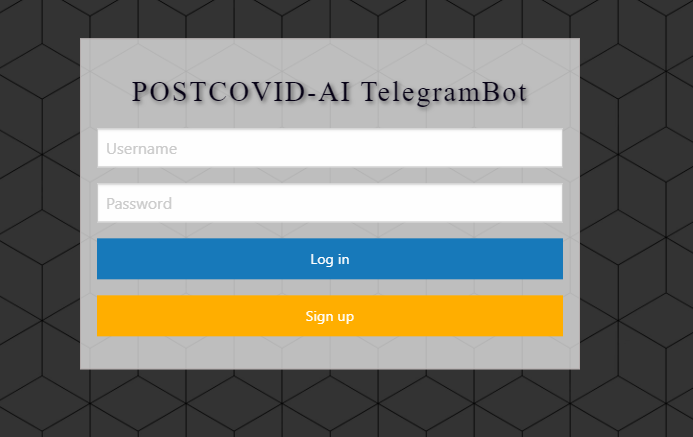
\includegraphics[width=0.8\textwidth, height=6cm]{imagenes/login.png}
    \caption{ Login usuarios }
    \label{fig:login}
\end{figure}

El login, que se ve en la \textit{\hyperref[fig:login]{Figura 5.3}}, es la primera página que se muestra cuando intentamos entrar. Solo pueden acceder a la aplicación los usuarios registrados.

En caso de no estar registrado se provee de un formulario para ello como se muestra en la \textit{\hyperref[fig:general]{Figura 5.4}} . Este rellena los campos de la tabla User que crea un nuevo registro de usuario en el sistema para que pueda autenticarse y acceder a él. Además otorga todos los permisos de administrador para que pueda realizar cualquier tipo de acción. \vspace{1cm}


\begin{figure}[!ht]
  \centering
  \begin{subfigure}{0.7\textwidth}
    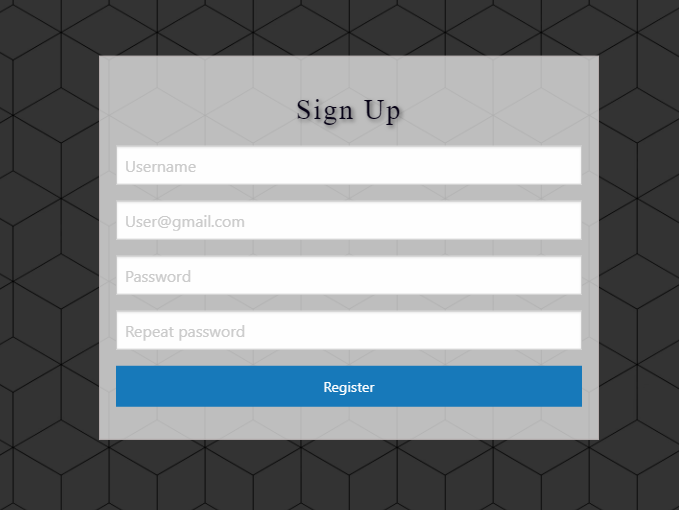
\includegraphics[width=\linewidth]{imagenes/register.png}
    \label{fig:imagen1}
  \end{subfigure}
  \hfill
  \begin{subfigure}{0.7\textwidth}
    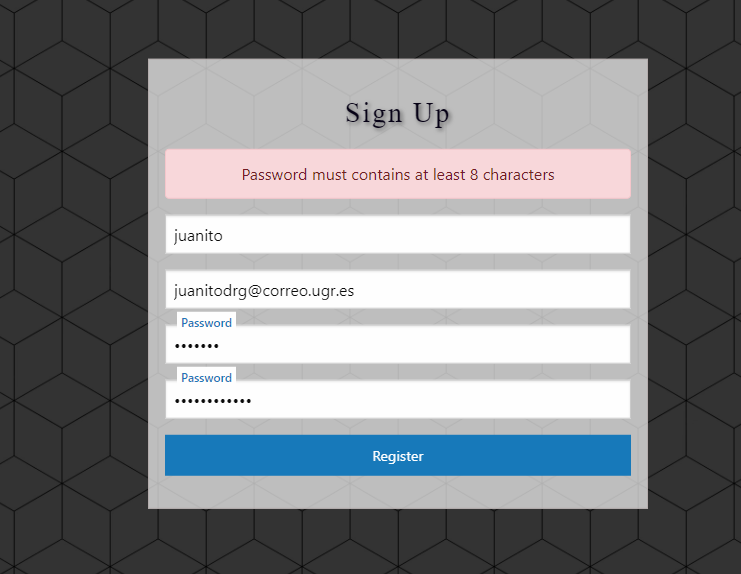
\includegraphics[width=\linewidth]{imagenes/register2.png}
    \label{fig:imagen2}
  \end{subfigure}

  \caption{Formulario de registro}
  \label{fig:general}
\end{figure}\vspace{2cm}

Cada usuario que desee registarse deberá especificar un username, email y la contraseña. El formulario cuenta con validaciones como que el nombre de usuario no se encuentre repetido en el sistema, escribir la contraseña dos veces y que coincidan o que esta tenga más de 8 caracteres. 

\subsection{Home}

Una vez logueados en el sistema, nos redirige al home. El home es la vista principal de la aplicación, la primera página que los usuarios ven cuando acceden al sitio web \textit{\hyperref[fig:home]{Figura 5.5}}. Proporciona información clave y navegación a otras secciones. Este consta de 4 secciones principales: Preguntas, Bloques, Preámbulos, Respuestas.\vspace{0.5cm}

\begin{figure}[!ht]
    \centering
    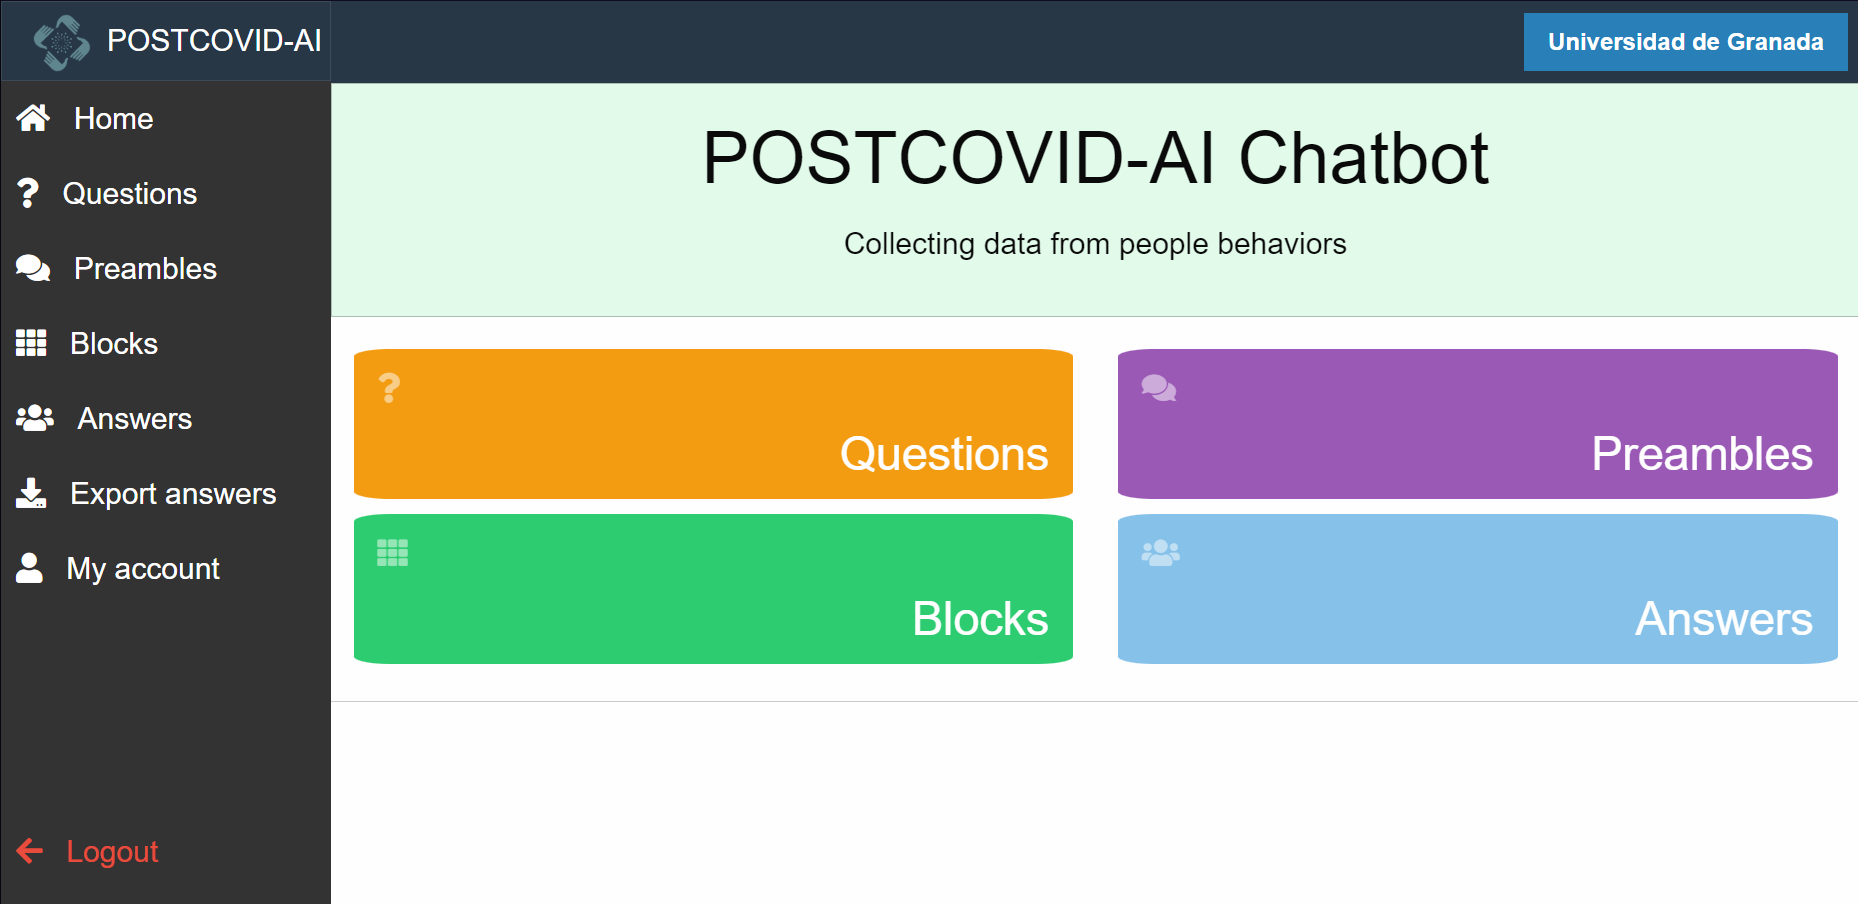
\includegraphics[width=1\textwidth, height=6cm]{imagenes/home2.png}
    \caption{ Home }
    \label{fig:home}
\end{figure}
\vspace{0.5cm}

Todas las vistas además cuentan con una barra lateral desplegable para realizar algunas operaciones de manera rápida como la redirección a las otras vistas, exportar respuestas, modificar la información del usuario y hacer logout. 

Por ejemplo, en la \textit{\hyperref[fig:modify-user]{Figura 5.6}} se muestra la vista de modificar usuario donde nos muestra un formulario con los datos del usuario que se encuentra activo y nos da la posibilidad de cambiar la contraseña, pudiendo proporcionar una nueva.\vspace{0.5cm} 

\begin{figure}[!ht]
    \centering
    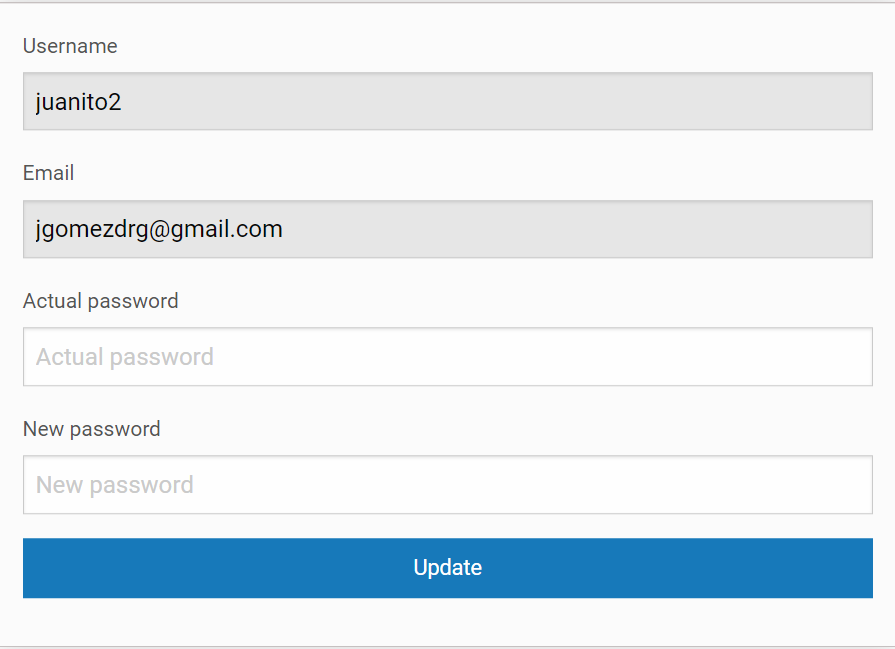
\includegraphics[width=0.5\textwidth, height=5cm]{imagenes/actualizacion_usuario.png}
    \caption{ Actualización usuario }
    \label{fig:modify-user}
\end{figure}\vspace{0.5cm} 




\subsection{Gestores}


Todas las secciones que veremos consisten en tablas paginadas que muestran la información guardada de cada registro pertenecientes a cada modelo. Además todas constan de un botón para añadir un nuevo registro, eliminar, modificar y clonar. \vspace{0.3cm}

Se ha implementado un buscador en cada una de las vistas de cada sección.

\begin{figure}[!ht]
    \centering
    
\includegraphics[width=0.5\textwidth]{imagenes/search.png}
    \caption{ Buscador }
    \label{fig:enter-label}
\end{figure}

Este buscador mostrará la lista de registros cuyos nombres coincidan con aquello escrito, para facilitar el acceso a la información deseada de manera más eficiente.

\subsection{Preguntas}


Dentro de la tabla de preguntas se muestra de forma general los campos mas relevantes para distinguirlas, mostrado en la \textit{\hyperref[fig:vista-preguntas]{Figura 5.8}}, como el enunciado, el bloque al que pertenecen, la fecha y el usuario que la ha creado. 

Como se ve en la parte superior derecha, se encuentra un botón para añadir una pregunta. Si navegamos por las filas de la tabla y clicamos en una se nos abrirá la vista para modificar la pregunta. Además en la parte derecha de cada fila hay un botón para eliminar el registro deseado.

\begin{figure}[!ht]
    \centering
    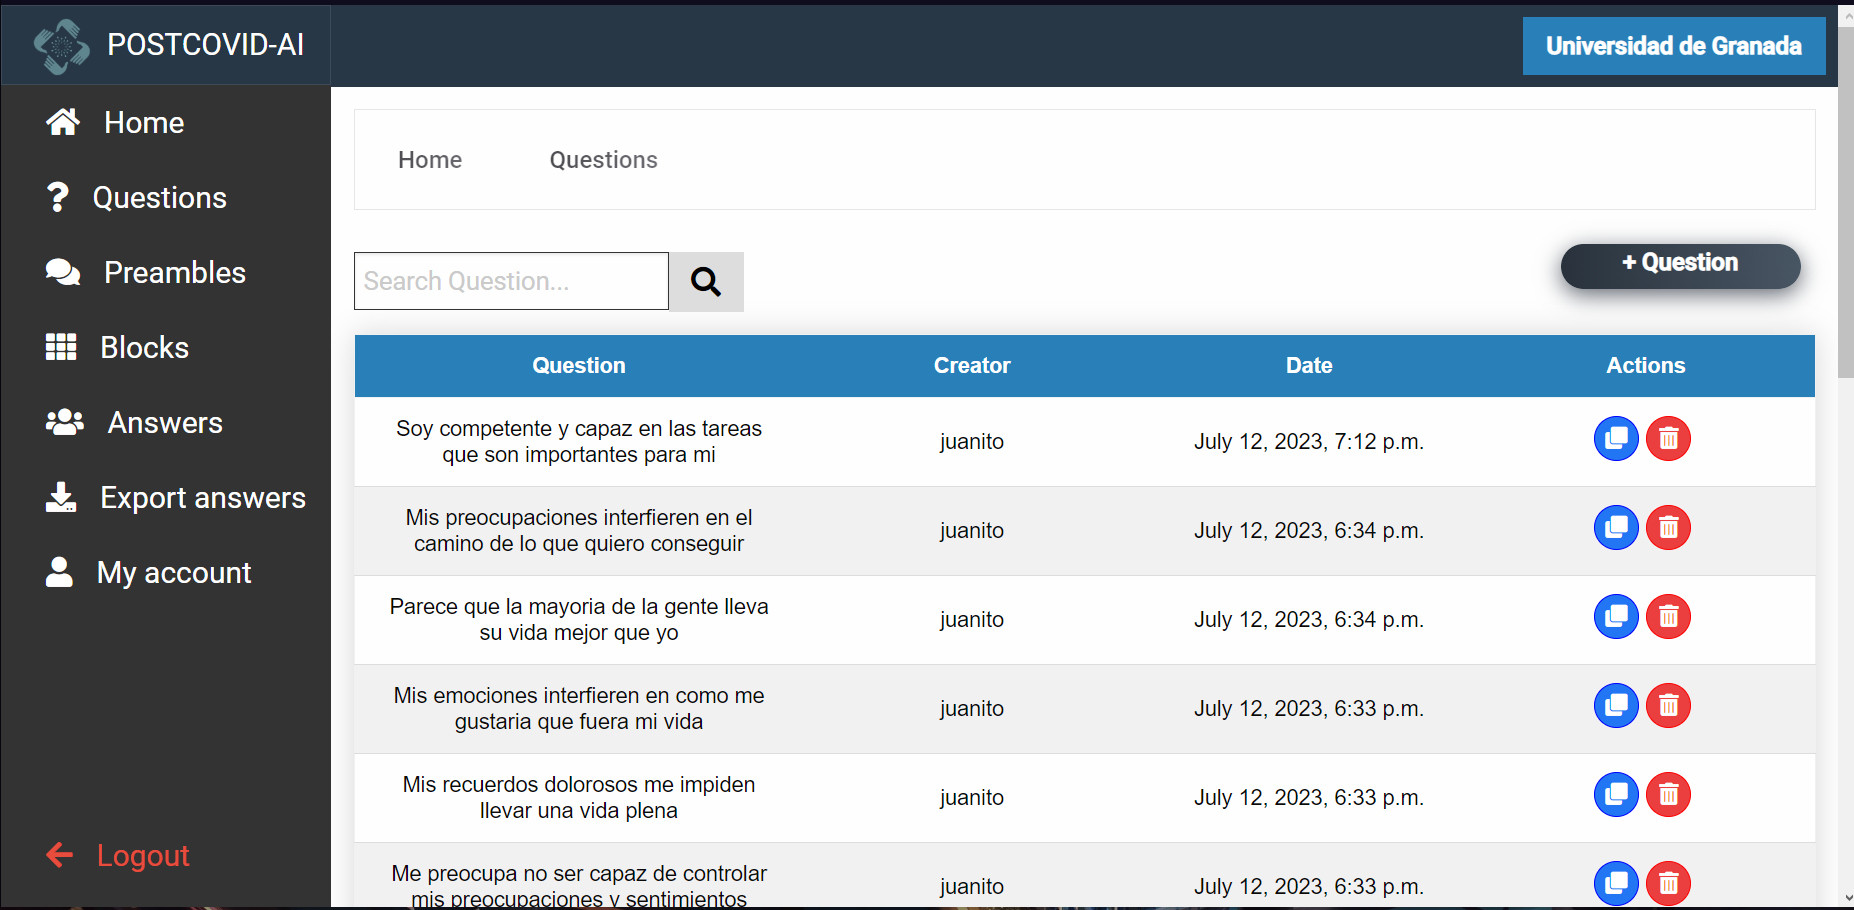
\includegraphics[width=1\textwidth]{imagenes/list_preguntas.png}
    \caption{ Listado de preguntas }
    \label{fig:vista-preguntas}
\end{figure}\vspace{0.5cm}

Si se pulsa en el botón para añadir una pregunta se abrirá una nueva página con un formulario con los datos necesarios para registrarla. A nivel de base de datos los campos que requiere cada pregunta son los siguientes:\vspace{0.3cm}

\begin{itemize}
    \item \textit{id}
    \item  \textit{title}: Enunciado de la pregunta.
    \item \textit{creator}: Foreign key a Usuario.
    \item \textit{date}: Fecha en la que se crea la pregunta. 
\end{itemize}\vspace{0.3cm}

El id como en todas las tablas es la clave primaria. A su vez, la pregunta tiene una clave externa a la tabla \textit{Posibles Respuestas}. Por lo que cada pregunta tiene varias posibles respuestas y cada posible respuesta tiene asignada una pregunta. En este caso, como se ve en la \textit{\hyperref[fig:add-question]{Figura 5.9}}, para registrar la pregunta solo se necesita proporcionar el titulo y las posibles respuestas ya que el campo de creador se autorellena con el usuario que la crea y en fecha se rellena con la actual.

Dentro del panel de posibles respuestas se deben añadir las respuestas a esa pregunta, cada una separada por línea. A su vez cuando se cree la pregunta también se crearán los registros de las respuestas asociadas a la pregunta. \vspace{1cm}

\begin{figure}[!ht]
    \centering
    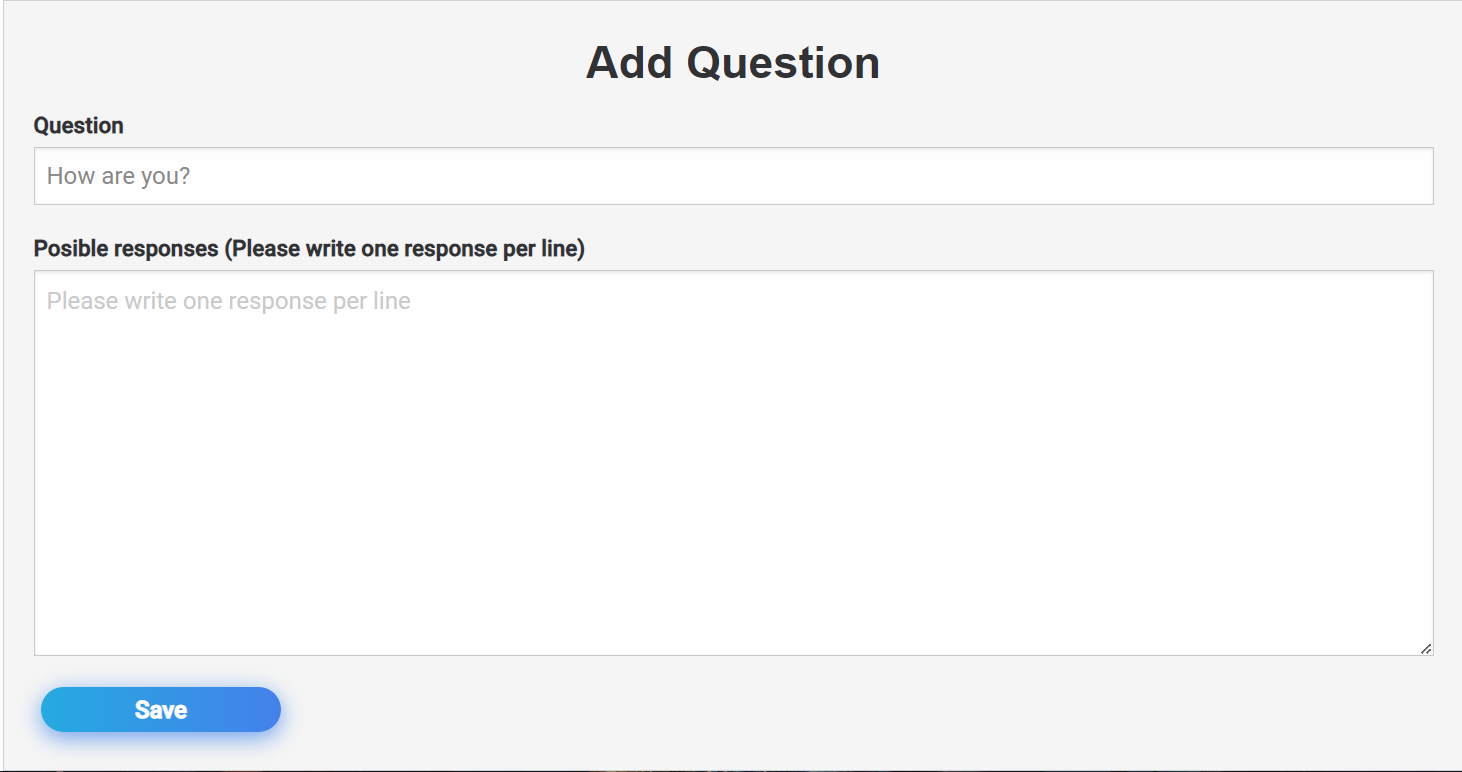
\includegraphics[width=1\textwidth]{imagenes/add_question.png}
    \caption{ Añadir pregunta}
    \label{fig:add-question}
\end{figure}\vspace{1cm}


En la \textit{\hyperref[fig:modify-question]{Figura 5.10}} se observa el formulario de modificación de la pregunta en el que se puede cambiar el titulo y las respuestas. Si otro usuario modifica la pregunta también se actualiza el campo del creador y fecha.

\begin{figure}[!ht]
    \centering
    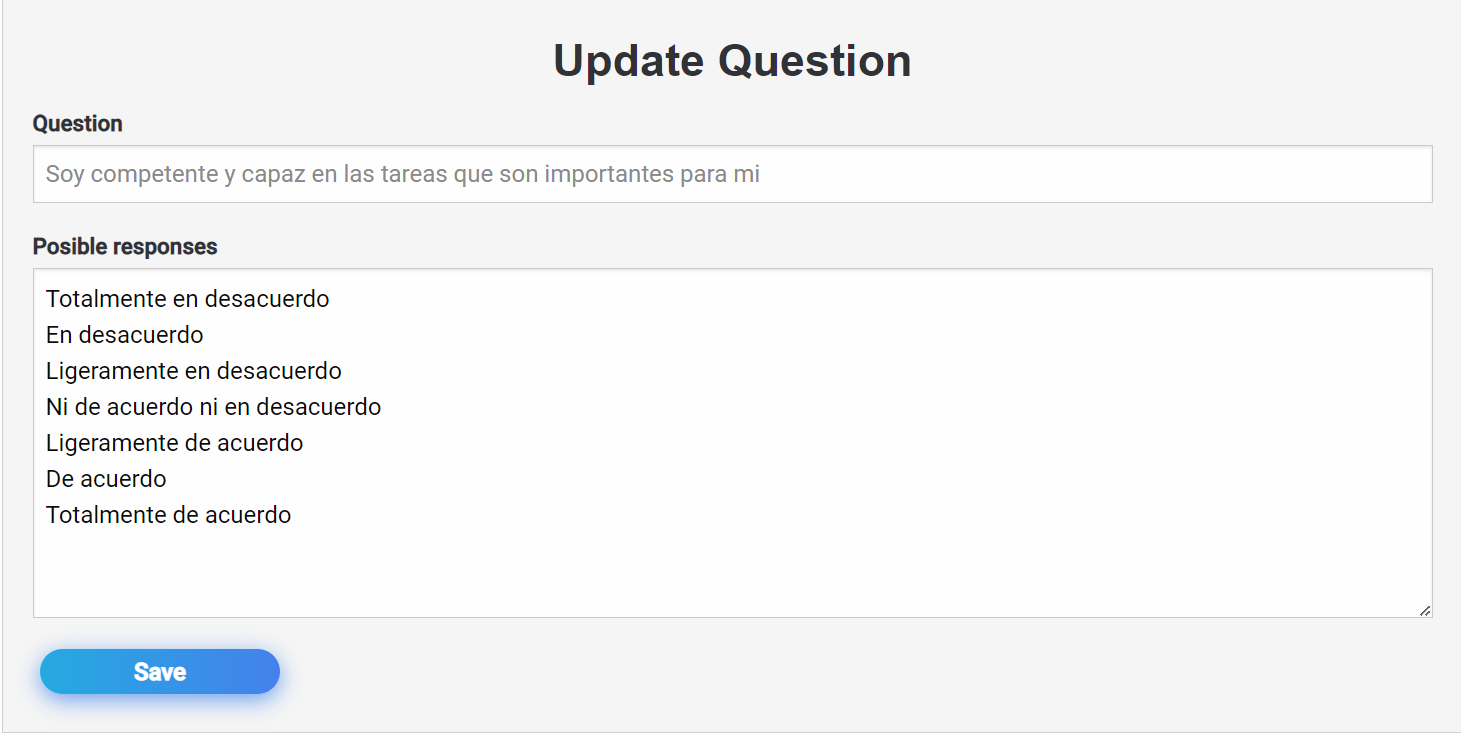
\includegraphics[width=1\textwidth]{imagenes/update_question.png}
    \caption{ Modificar Pregunta}
    \label{fig:modify-question}
\end{figure}\vspace{0.5cm}


También se pueden eliminar y clonar preguntas, tal como se ve en la \textit{\hyperref[fig:vista-preguntas]{Figura 5.7}}. Concretamente, si se selecciona el botón de eliminar (que se ve como un símbolo de papelera rojo a la derecha de cada fila), aparecerá una alerta para verificar si realmente se desa borrar la pregunta \textit{\hyperref[fig:delete-question]{(Figura 5.11)}} y en caso afirmativo se realiza. También vemos un botón azul justo al lado, que es el botón de clonar. Este botón creará una nueva pregunta idéntica a la seleccionada.

\begin{figure}[!ht]
    \centering
    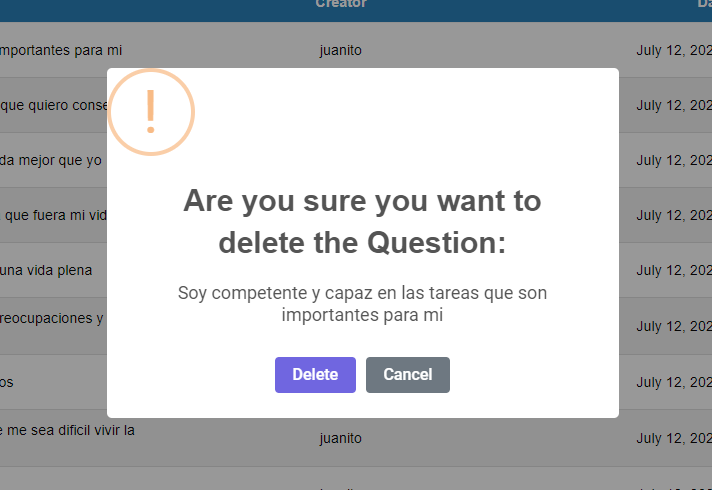
\includegraphics[width=0.7\textwidth, height=7cm]{imagenes/delete_question.png}
    \caption{ Borrar Pregunta}
    \label{fig:delete-question}
\end{figure}


\subsubsection{Bloques}\vspace{0.5cm}

\begin{figure}[!ht]
    \centering
    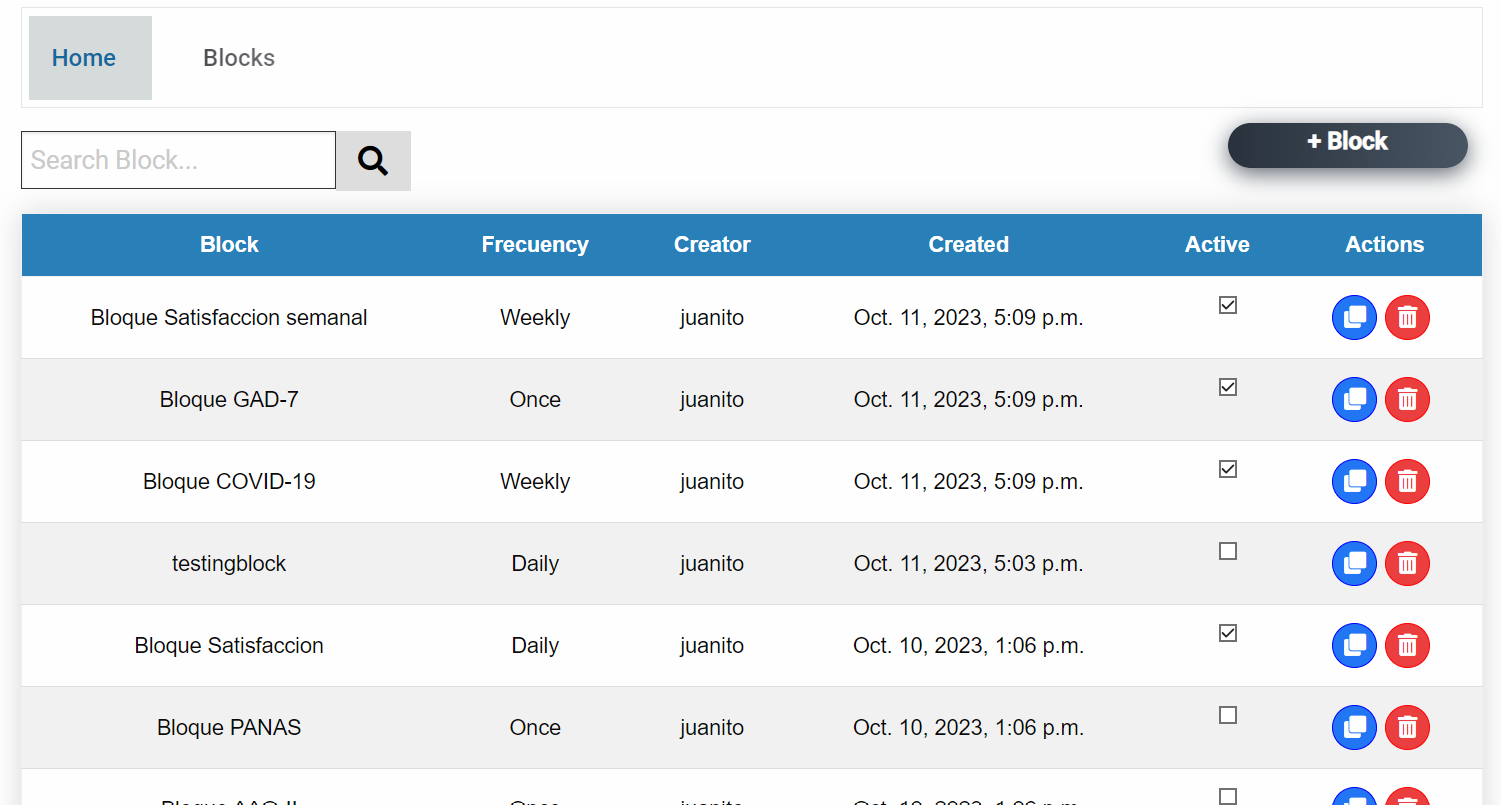
\includegraphics[width=1\textwidth]{imagenes/list_bloques.png}
    \caption{Listado de Bloques}
    \label{fig:lista-bloques}
\end{figure}

La \textit{\hyperref[fig:lista-bloques]{Figura 5.12}} muestra la tabla que contiene los registros de los bloques de preguntas en el sistema. Al igual que en la vista anterior cuenta con las operaciones de añadir, modificar y eliminar un bloque. 

Los campos necesarios para registrar un bloque en la base de datos son los siguientes: \vspace{0.3cm}

\begin{itemize}
    \item \textit{id}
    \item \textit{block}: Nombre del bloque.
    \item \textit{active}: Atributo que indica si el bloque se encuentra activo.
    \item \textit{operating}: Indica si el bloque se encuentra operando en ese momento.
    \item \textit{questions}: Foreign Key a Pregunta.
    \item \textit{preamble}: Foreign key a Preámbulo.
    \item \textit{frecuency}: Frecuencia del bloque.
    \item \textit{time}: Hora de la planificación.
    \item \textit{day}: Día de la planificación.
    \item \textit{duration}: Duración activa del bloque.
    \item \textit{creator}: Foreign key a Usuario.
    \item \textit{date}: Fecha en la que se crea el bloque.
\end{itemize}

El campo \textit{questions} es una relacion de tipo \textit{ManyToMany} con la tabla de preguntas. Un mismo bloque tendrá la posibilidad de asignar el número de preguntas que desee. Todas esas preguntas a su vez pertenecerán a ese bloque.  


\begin{figure}[!ht]
    \centering
    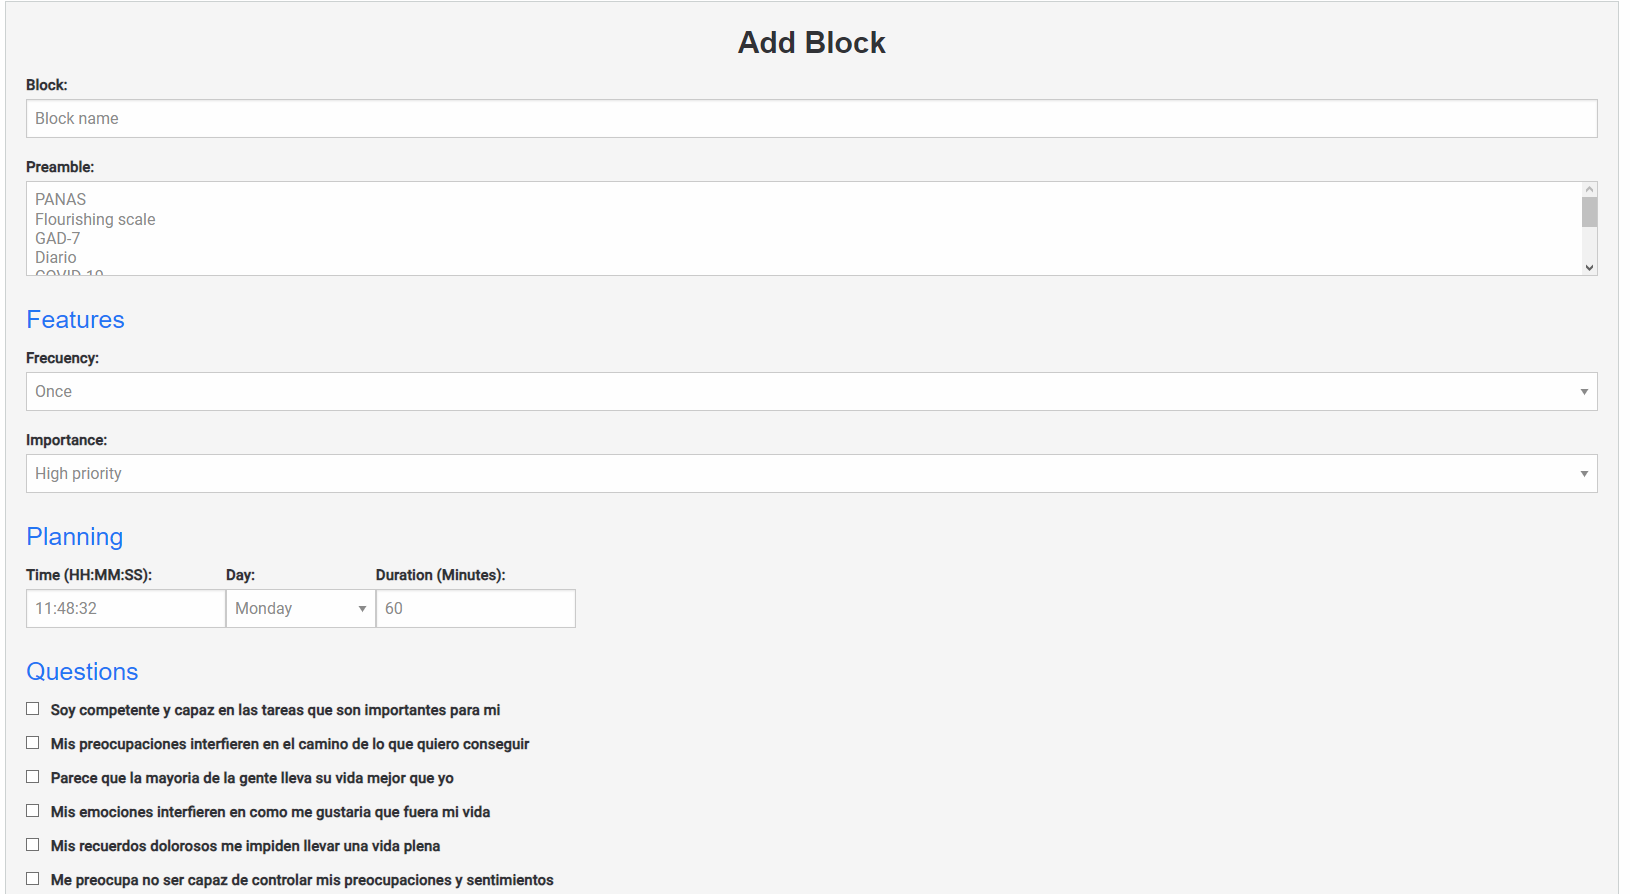
\includegraphics[width=1\textwidth, height=6cm]{imagenes/aniadir_bloque.png}
    \caption{Añadir bloque}
    \label{fig:add-bloque}
\end{figure}

Como se ve en la \textit{\hyperref[fig:add-bloque]{Figura 5.13}}, se puede elegir mediante un checkbox las preguntas que se desee añadir y un recuadro en el que  muestra una lista de los preámbulos creados en el sistema, para elegir uno y asignarlo al bloque.


Una vez se han añadido preguntas al bloque y se le ha asignado un preámbulo, faltaría definir la frecuencia del bloque, su importancia y el atributo activo. Estos atributos están más relacionados con el bot. La frecuencia define cada cuanto tiempo se debe realizar el cuestionario asociado al bloque. Normalmente, las preguntas dentro de un mismo bloque tienen un sentido y un propósito común. Por ejemplo, hay preguntas sobre salud, horas de sueño, alimentación que necesitan de realizarse todos los días o una vez por semana. Mientras que hay otras que con solo hacerse una vez ya bastaría. De ahí nace la idea de agrupar las preguntas en bloques. Dentro de la frecuencia puede elegir entre:

\begin{itemize}
    \item Once
    \item Daily
    \item Weekly
\end{itemize}

Otro campo sería la importancia del bloque (High importance, Normal, Low importance). Este campo  se añadió para que a la hora de que el bot haga el cuestionario de un bloque, priorice los de mayor importancia ante los otros. El atributo activo va a definir la disponibilidad de ese bloque, es decir, si este se encuentra seleccionado, el bloque estará activo para los usuarios y este se ejecutará dependiendo de su planificación, pero si se encuentra inactivo nunca se realizará el cuestionario asociado (cuando se crea un bloque por defecto está desactivado, solo se activará marcando la casilla). Ahora vendría la planificación del bloque. Una de las finalidades de este trabajo es el diseño y desarrollo de un sistema de cuestionarios dinámicos, que permite a los usuarios planificar la fecha y hora de activación de los bloques, así como definir la duración de los mismos. El sistema proporciona flexibilidad y adaptabilidad para ajustar estos parámetros, permitiendo una personalización efectiva de la experiencia del usuario. Para ello se proporcionan los atributos de \textit{time, day, duration} de forma que se pueda automatizar este proceso. 


\begin{figure}[!ht]
    \centering
    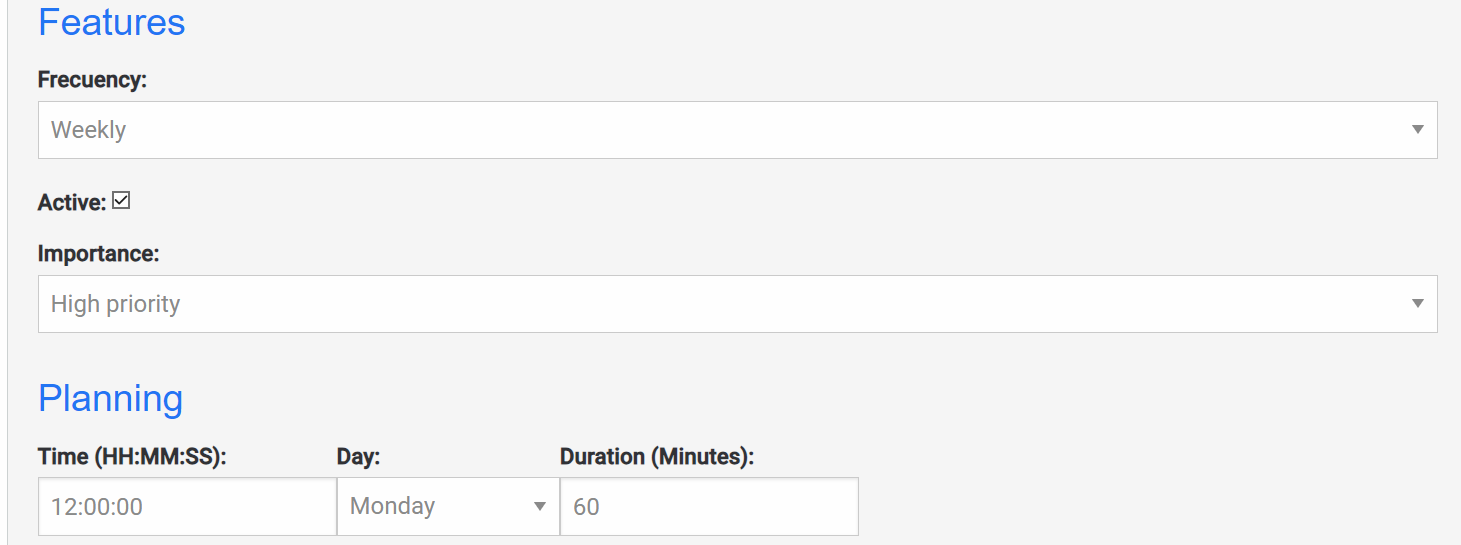
\includegraphics[width=1\textwidth, height=4cm]{imagenes/plan_bloque.png}
    \caption{Planificación Bloque}
    \label{fig:planificacion_bloque}
\end{figure}

En la figura \textit{\hyperref[fig:planificacion_bloque]{Figura 5.14}}, se puede ver como sería el ejemplo de planificar un bloque una vez a la semana todos los miércoles a las 12:00 horas y con una duración activa de 60 minutos.\vspace{0.3cm}

\subsubsection{Preámbulos}

Los preámbulos contienen los mensajes a mostrar por parte del bot en el chat del usuario cuando se va a tratar un tema concreto. Cuando se entra en un bloque el bot muestra un mensaje a forma de introducción que nos pone en contexto acerca del tema a tratar en el cuestionario. Esta tabla se crea como idea para que haya variedad a la hora de mostrar estos mensajes introductorios. \vspace{0.7cm}

\begin{figure}[!ht]
    \centering
    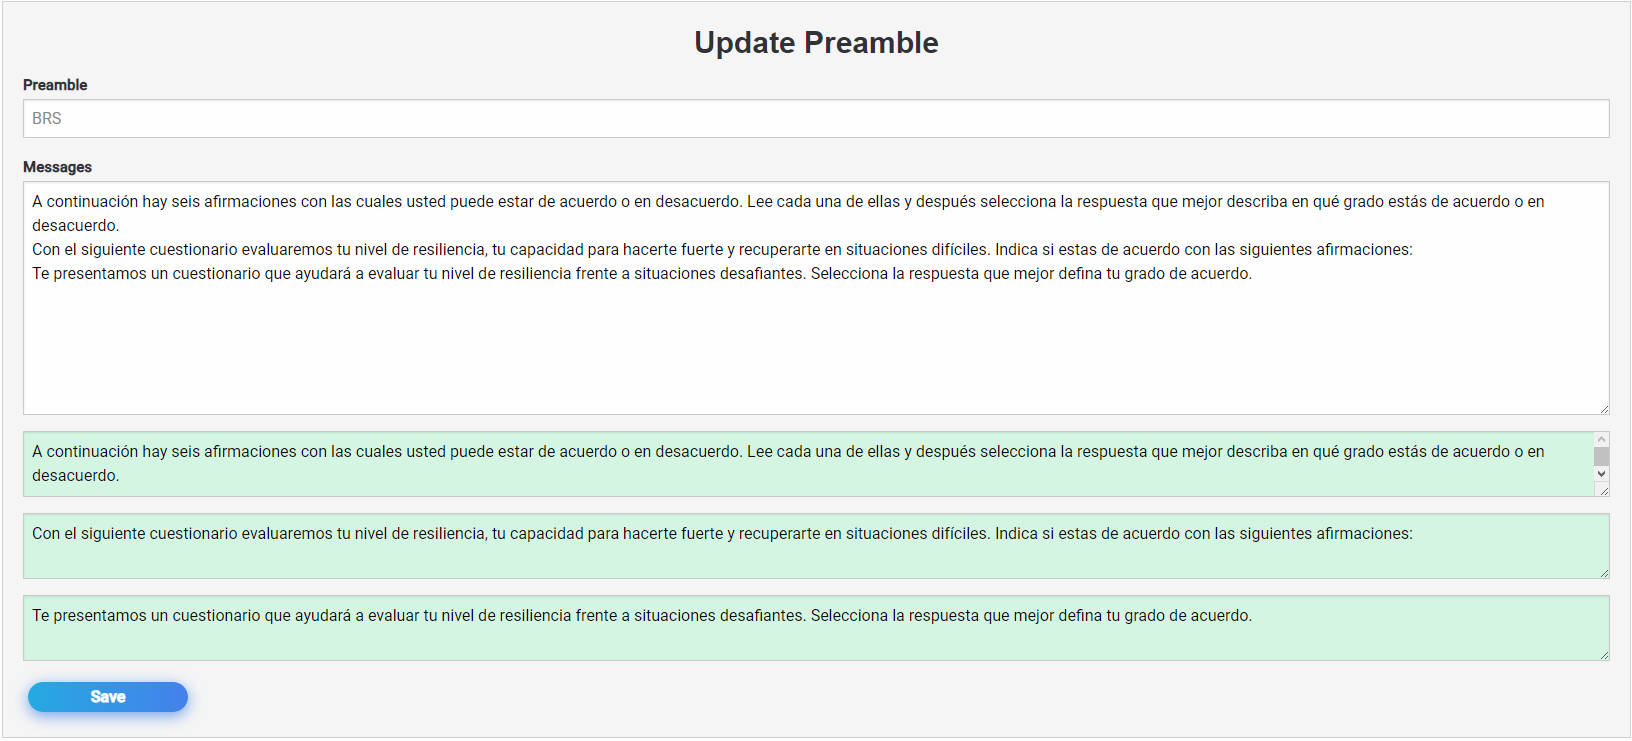
\includegraphics[width=1\textwidth]{imagenes/update_preamble.png}
    \caption{Editar Preámbulo}
    \label{fig:update-preamble}
\end{figure}\vspace{0.7cm}

En la \textit{\hyperref[fig:update-preamble]{Figura 5.15}} se puede ver un ejemplo que nos aclara con mayor detalle la función del preámbulo. El tema es AAQ-II, estas preguntas sirve para evaluar el nivel de aceptación psicológica y disposición a actuar de una persona. Cuando se realice el cuestionario asociado se mostrará uno de los tres mensajes que dispone. 

La forma de crearlos es parecida a la de las preguntas que se explica previamente. Existen 2 tablas: \textit{Preámbulos} y \textit{Mensajes}. La clase preámbulo contiene los nombres, y la de mensajes los enunciados de la información a mostrar, que tienen una clave foránea a preámbulo.\vspace{1.5cm}

\textbf{Clase Preámbulo:}

\begin{itemize}
    \item \textit{name}: Nombre.
\end{itemize}

\textbf{Clase Mensaje}

\begin{itemize}
    \item \textit{text}: Enunciado del mensaje.
    \item \textit{preamble}: Foreign key a Preámbulo.
\end{itemize}


Para crearlo se especifica el nombre y los mensajes, cada uno separado por una línea, que crea todos los registros y los asocia al preámbulo actual.\vspace{0.5cm}

\subsubsection{Respuestas}

Por último nos encontramos el apartado de respuestas, mostrado en la \textit{\hyperref[fig:list-answers]{Figura 5.16}}. Esta vista es simplemente a modo de visualización ya que el administrador no podrá realizar operaciones con ellas. Estas se crean automáticamente cuando un usuario responde a la pregunta hecha por el bot. 

\begin{figure}[!ht]
    \centering
    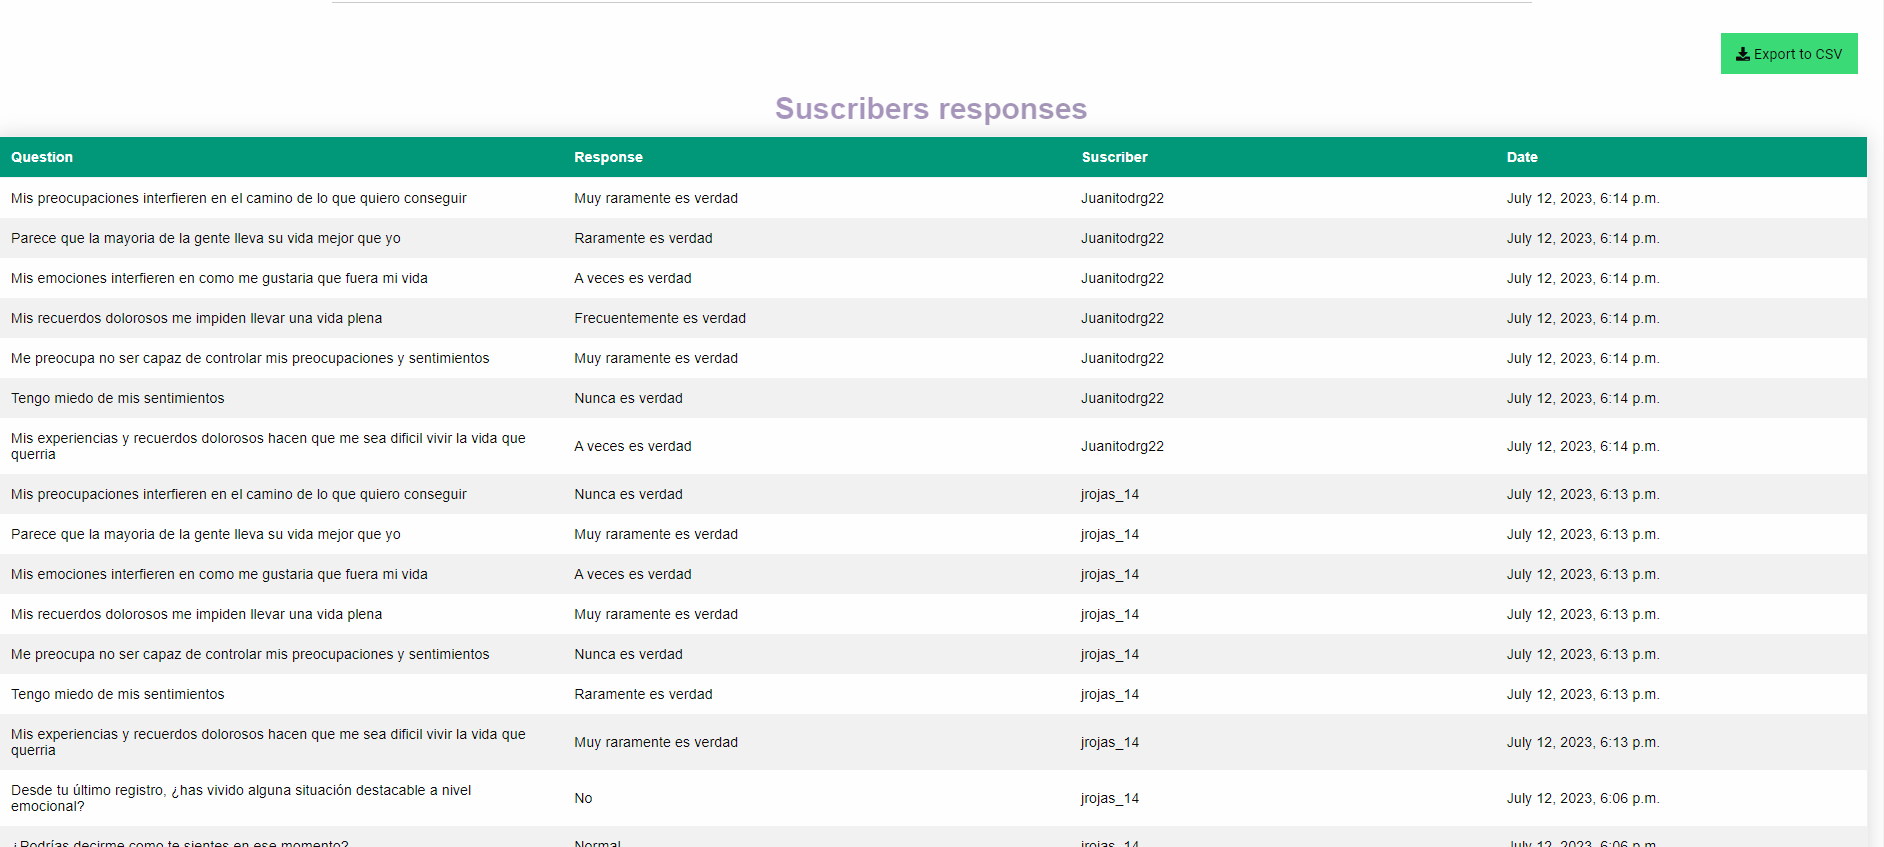
\includegraphics[width=1\textwidth]{imagenes/list_answers.png}
    \caption{Lista respuestas}
    \label{fig:list-answers}
\end{figure}


Los campos para registar una respuesta son los siguientes:

\begin{itemize}
    \item \textit{id}
    \item \textit{block}: Foreign key a Bloque.
    \item \textit{question}: Foreign key a Pregunta.
    \item \textit{response}: Respuesta del usuario.
    \item \textit{suscriber}: Foreign key a Usuario.
    \item \textit{date}: Fecha de la Respuesta.
\end{itemize}

Esta vista cuenta además con un botón en la parte superior derecha para exportar las respuestas a formato CSV. Los archivos CSV almacenan los datos separados con comas, por lo que cuando se guarda el texto y los números es fácil moverlos de un programa a otro. Al fin y al cabo este es el propósito de nuestro proyecto, recaudar información y entregarla en un formato específico para que el análisis sea sencillo.

La función que lo realiza es la siguiente:

\begin{lstlisting}[language=Python]
def export_to_csv(request):
    answers = Answer.objects.all()
    buffer = io.StringIO()
    writer = csv.writer(buffer, delimiter=';')

    writer.writerow([smart_str('Block'), smart_str('Question'), smart_str('Response'), smart_str('Subscriber'), smart_str('Date')])
    
    for answer in answers:
        block = smart_str(answer.block.block)
        question = smart_str(answer.question.title)
        response = smart_str(answer.response)
        subscriber_username = smart_str(answer.suscriber.username)
        date = smart_str(answer.date.strftime('%Y-%m-%d'))

        writer.writerow([block, question, response, subscriber_username, date])
    
    csv_file_name = 'answers_export.csv'
    with open(csv_file_name, 'w', encoding='latin1') as csv_file:
        csv_file.write(buffer.getvalue())
    
    with open(csv_file_name, 'rb') as csv_file:
        response = HttpResponse(csv_file.read(), content_type='text/csv')
        response['Content-Disposition'] = f'attachment; filename={csv_file_name}'
    
    return response
\end{lstlisting}

Python cuenta con una librería llamada csv. Esta librería implementa clases para leer y escribir datos tabulados en formato CSV.\vspace{0.5cm}


\section{Chatbot}


El agente conversacional se encuentra formado por 3 módulos diferenciados: Módulo de bienvenida y registro de usuario, módulo conversacional y cuestionario.

\subsection{Módulo de bienvenida y registro}

La libreria \textit{python-telegram-bot} es la herramienta con la que vamos a interactuar con la API de Telegram. La librería emerge como una herramienta indispensable en este ámbito, proporcionando a los desarrolladores un marco completo para construir, desplegar y gestionar bots de Telegram sin esfuerzo.

Esta nos va a permitir diferentes posibilidades a la hora de crear nuestro bot como son la gestión de actualizaciones para controlar diferentes tipos de entradas de manera eficiente, envío de mensajes de texto y contenido multimendia, teclados y botones, comandos personalizados, respuestas interactivas, middleware y filtros. Todo lo relacionado a la descripción de estas operaciones se encuentra especificado en la documentación oficial \textit{(\cite{pythontelegrambot})}.

Este primer módulo tiene como objetivo la presentación de nuestro bot con el usuario y su registro en nuestra base de datos. Contiene una función que es la primera que se ejecuta cuando cualquier persona empieza una conversación. Se activa con el comando \textit{/start} que se envía mecánicamente y es el único comando necesario para la conversación. Cuando este evento se detecta se realiza una llamada a la función la cual muestra un mensaje de bienvenida al usuario presentando los temas a tratar. Gracias a la librería usada podemos obtener los datos que el usuario posea en su Telegram personal (como el nombre, nombre de usuario, apellidos, email, id).\vspace{0.3cm}

\begin{lstlisting}[language=Python]
    suscriber, created = Suscriber.objects.get_or_create(
        chatid = chat_id,
        name=name,
        surname=surname,
        username=username,
    )
\end{lstlisting}

 La función de Django \textit{get\_or\_create()} nos permite filtrar una serie de datos introducidos dentro de una tabla en la base de datos. En caso de que ningún registro coincida exactamente con todos los datos, crea una nueva instancia con los parámentros pasados. De esta forma se registran los usuarios. Para asegurarnos de la concurrencia de nuestro programa, se ha creado un atributo en usuario llamado \textit{chatid} que almacena el id propio del chat. Esto se hace con la intención de no declarar variables globales dentro del código ya que si hubiera varias personas hablando al mismo tiempo habría problemas de concurrencia. Por eso cada consulta y cada mensaje es específico para cada uno intentando operar siempre desde la base de datos, lo que además influye positivamente en la eficiencia ya que las consultas y operaciones son más rápidas.


\begin{figure}[!ht]
    \centering
    
\includegraphics[width=0.8\textwidth, height=4cm]{imagenes/welcome.png}
    \caption{ Mensaje de bienvenida }
    \label{fig:welcome}
\end{figure}

La figura \textit{\hyperref[fig:welcome]{Figura 5.17}} muestra como es el mensaje de presentación del bot. Nos pone en contexto y nos habla sobre su propósito. Finalmente nos hace una pregunta y dependiendo de la respuesta del usuario nos redigirá a un módulo u otro. 



\subsection{Módulo conversacional}

Este módulo es una etapa intermedia, que funciona como una especie de sala de espera a que el usuario cuente con cuestionarios a responder. Dentro de él, se puede tener una conversación de lo más común y simple con el bot, con un apartado que muestra preguntas frecuentes en caso de que el usuario tenga cualquier tipo de duda. 

El usuario puede entrar dentro de este módulo de diferentes maneras. Una de ellas es respondiendo de forma negativa en la pregunta anterior. Dentro de este módulo hay unas palabaras, frases o expresiones previamente definidas por las cuales el bot responde en función de lo que escribas. Cabe destacar que no se utiliza modelos de lenguaje como GPT (Generative Pre-Trained Transformer) para generar respuestas mas elaboradas. GPT es un modelo que utiliza algoritmos avanzados de procesamiento de lenguaje natural para generar respuestas a preguntas y comentarios de los usuarios en tiempo real \textit{(\cite{gpt2020})}. En nuestro caso esa no es la finalidad de nuestro bot. Como ya se ha indicado el propósito principal es la recogida de datos, con la funcionalidad añadida de que el usuario pueda tener una conversación escueta con el bot para que esta recogida se realice de la forma más humanamente posible, pero esta quedando siempre en segundo plano. 

Este módulo se ejecuta de forma recursiva cada vez que el usuario escribe un mensaje en el chat. Funciona de la siguiente manera:\vspace{0.3cm}

\textbf{1. Recogida del mensaje: }Cuando el usuario manda cualquier tipo de mensaje el bot lo recibe como texto de entrada y lo almacena.\vspace{0.3cm}

\textbf{2. Procesamiento: }Este proceso implica limpiar y normalizar el texto introducido, convirtiéndolo a minúsculas y reduciendo las palabras a su forma base. \vspace{0.3cm}

\textbf{3. Análisis: }Conlleva la identificación del contexto del mensaje con el propósito de extraer información relevante o identificar intenciones. 

Esta identificación se hace dentro del archivo \textit{replyMessages.py} situado dentro de la carpeta /chatbot. En el podemos encontrar diferentes listas como estas.\vspace{0.5cm}

\begin{lstlisting}[language=Python]
#HELLO AND GOOD BYE
greetings = ['hola', 'hello', 'buenos dias', 'buenas tardes', 'buenas', 'saludos', 'hi', 'good']
farewell = ['adios', 'bye', 'good bye', 'hasta luego', 'nos vemos', 'hasta pronto', 'buenas noches', 'que tengas un buen dia', 'hasta la proxima','que vaya bien']

\end{lstlisting}

Este es un ejemplo de lista para establecer el contexto de saludo y despedida. Estas listas definen una serie de palabras y expresiones concretas que cualquier persona hispanohablante utilizaría si quisiera referirse o hablar sobre un tema. Si cualquier palabra dentro de la respuesta del usuario se encuentra contenida en esta lista el bot identifica la intención del mensaje y le asociará un contexto.\vspace{0.3cm}

\textbf{4. Generación de respuesta: }Una vez encontrado el contexto del mensaje debemos buscar una respuesta digna que se adecue al tema tratado. Para ello dentro de este mismo archivo mencionado encontramos varios diccionarios. Estos contienen las respuestas que el bot debe proporcionar para cada contexto. Por ejemplo:

\begin{lstlisting}[language=Python]
    'greetings':{
        '0': 'Hola!¿Puedo ayudarte en algo?',
        '1': 'Muy buenas!¿Necesitas ayuda?',
        '2': 'Hola!¿Como puedo asistirte hoy?'
    },
    'farewell':{
        '0': '¡Adios!.¡Que tengas un buen dia!',
        '1': 'Hasta luego!.¡Espero verte de nuevo pronto!',
        '2': 'Adios. !No dudes en volver!',
    },
\end{lstlisting}

Cuando declaramos el contexto de saludo como este ejemplo, vemos que hay una serie de mensajes. He intentado que haya un mínimo de unos tres mensajes por cada contexto para que la respuesta proporcionada por el bot no sea siempre igual e intentar que esta varie. A la hora de mostrarlo en el chat se hace con la función que se muestra a continuación, la cual envía el mensaje al usuario concreto que lo ha escrito y selecciona una respuesta aleatoria dentro de las que el diccionario disponga.\vspace{0.3cm}

\begin{lstlisting}[language=Python]
context.bot.send_message(chat_id=user.id, text=messages['greetings'][str(random_var)])
\end{lstlisting}

Por último debemos tratar que pasaría si el bot no reconoce el mensaje del usuario, ya sea por hablar de un tema que el bot no tiene respuesta o por escribir mal una palabra o expresión. En este caso, en la etapa anterior de análisis el bot no podría clasificar la respuesta. Cuando esto sucede se muestra lo que vemos en la \textit{\hyperref[fig:no-entendido]{Figura 5.18}}.

\begin{figure}[!ht]
    \centering
    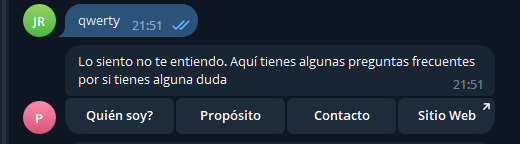
\includegraphics[width=1\textwidth]{imagenes/no_respuesta.png}
    \caption{Respuesta del bot a un mensaje no entendido}
    \label{fig:no-entendido}
\end{figure}\vspace{0.3cm}

El mensaje contiene botones con algunas preguntas frecuentes que puedan ser de interés al usuario (como información sobre el bot, su propósito, sitio web y contacto del proyecto a que pertenece). En la \textit{\hyperref[fig:faq]{Figura 5.19}} se pueden ver los mensajes que se mostrarían si se pulsa cada uno de los botones:

\begin{figure}[!ht]
    \centering
    
\includegraphics[width=0.7\textwidth, height=4cm]{imagenes/preguntas_frecuentes.png}
    \caption{ Respuestas del bot a las preguntas frecuentes }
    \label{fig:faq}
\end{figure}

\subsubsection{Calendario de cuestionarios}

Desde el momento que se ejecuta el programa se crea un proceso recursivo dentro del mismo para cada uno de los bloques registrados en el sistema. Este proceso se ejecuta de forma ininterrumpida dependiendo de la planificación que le hayamos dado a cada bloque. Es decir, si un bloque concreto se encuentra planificado para que se repita de forma diaria a las 14:00 horas, todos los días de la semana a esa hora en concreto se ejecutará el proceso. Este avisará a todos los usuarios registrados de que cuentan con un cuestionario activo y que pueden pasar a responderlo. Esto se hace mediante la ayuda de la libreria \textit{apscheduler}, que permite planificar procesos y ejecutarlos en tiempos determinados. Los denomina como 'Job'.

\begin{lstlisting}[language=Python]
    self.scheduler.add_job(
                self.advise,
                replace_existing=True,
                trigger=CronTrigger(day_of_week=self.block.days, hour=self.block.time.hour, minute=self.block.time.minute, second=self.block.time.second, timezone=pytz.timezone('Europe/Madrid')),
                id=str(self.block.id),
                name=self.block.block,
            )
\end{lstlisting}

Esta es la manera de crearlos, que como se ve en el código depende totalmente de la planificación del bloque. Lo que hace es llamar a otro método que muestra el mensaje mostrado en la \textit{\hyperref[fig:pending]{Figura 5.20}} al usuario y activa el cuestionario correspondiente. 

\begin{figure}[!ht]
    \centering
    
\includegraphics[width=1\textwidth]{imagenes/active_quest.png}
    \caption{ Mensaje cuestionario pendiente }
    \label{fig:pending}
\end{figure}


Los cuestionarios cuentan con una duración definida en cada bloque. Estos solo se encontrarán activos durante el tiempo que hayamos proporcionado (puede ser 30 minutos, 1 hora, 2 horas...). Cuando un cuestionario se activa en su momento planificado, lanza otro 'Job' que se ejecutará una vez pasado el tiempo de duración del bloque con la función de desactivarlo. De esta manera, si un cuestionario esta planificado, por ejemplo, el lunes a las 12:00 horas y tiene una duración de una hora, el bot avisará de que se cuenta con un cuestionario activo y todos los usuarios tendrán exactamente una hora para responderlo. Pasada esta hora el cuestionario se cierra y hasta la siguiente planificación no se podrá volver a responder.

También debemos de tener en cuenta cuando se modifique, se cree o se borre un bloque. Para ello el programa cuenta con un proceso interno que se ejecuta cada 30 segundos que ejecuta el siguiente método:

\begin{lstlisting}[language=Python]
    def actualize(context):
    global aux_blocks
    current_blocks = list(QuestionBlock.objects.all().values('id'))
    id_list1 = [item['id'] for item in current_blocks]
    id_list2 = [item['id'] for item in aux_blocks]
    different_blocks = list(set(id_list1) ^ set(id_list2))
    if different_blocks is not None:
        for item in different_blocks:
                try:
                    block = QuestionBlock.objects.get(id=item)
                    ScheduleJob(context, block, scheduler)

                except:
                    ScheduleJob.remove_schedule(context, str(item))

    aux_blocks = current_blocks
\end{lstlisting}

La función de este método es buscar modificaciones en la base de datos y actualizar los calendarios. En el caso de crear un nuevo bloque creará un nuevo calendario, al borrar un bloque existente eliminará su calendario asociado con el fin de que no se ejecute más, o al modificarlo actualizará el actual.


\subsection{Módulo cuestionario}


Pasamos ahora al último módulo de nuestro bot. Este módulo sigue el ejemplo de un cuestionario de preguntas clásico en el que el bot va haciendo una serie de preguntas y se debe responder con una de las opciones posibles conforme al criterio de cada uno. 

Para entrar, el bot ya sea al principio o cuando se cuente con preguntas pendientes, se hará la pregunta de si se quiere comenzar el cuestionario. Solo se entrará en él cuando se responda de forma afirmativa a esta pregunta. Una vez estemos dentro, el bot explicará de forma escueta como funciona y eligirá la primera pregunta. He aquí cuando entra en juego una de las funciones principales \textit{chooseQuestion(user)}.

\begin{lstlisting}[language=Python]
def choose_question(user):
    global first
    first = False
    bloques = QuestionBlock.objects.filter(operating=True, active=True).order_by('-importance')
    block_counter = 0
    question_result = []
    for block in bloques:
        questions = Question.objects.filter(blocks=block).order_by('create')
        first_value = questions.first()
        for question in questions:
            if is_answered(user, question, block) == False:
                question_result.append(question)
                question_result.append(block)
                if question == first_value:
                    first = True
                break
        block_counter += 1
    return question_result
\end{lstlisting}

Esta función recorre los bloques de preguntas que se encuentran activos en el sistema ordenándolos por importancia. Comprueba las preguntas una a una dentro de cada bloque filtrando las respuestas para cada usuario y comprobando si ha sido respondida. En este punto tenemos dos posibilidades. Que el usuario sea nuevo y no ha realizado ningún cuestionario, por lo que la primera pregunta que compruebe será la devuelta ya que no hay ningún registro de respuestas por su parte. Y en caso contrario, que el usuario ya haya realizado varios cuestionarios. En este supuesto, se resolvería de la misma forma que el Job entiende cuando un usuario cuenta con preguntas pendientes, es decir, comparando las fechas de las respuestas con la fecha actual, restándola y si es mayor a la frecuencia del bloque, significa que esa pregunta se encuentra pendiente, si no pasaría a la siguiente. Además el método identifica la primera pregunta perteneciente a cada bloque, para que cuando esta se ejecute muestre cualquiera de los mensajes asociados al preámbulo de ese bloque de preguntas.

Para el cuestionario, se ejecuta recursivamente la función \textit{handleanswer(update, context)} que es la encargada de realizar las preguntas, separándolas por bloques, mostrar los mensajes asociados a los preámbulos y recoger las respuestas como lo vemos en la \textit{\hyperref[fig:cuestionario]{Figura 5.21}}. Solo termina cuando el usuario no cuente con preguntas pendientes. En cada iteracción hace una llamada a la función anterior \textit{chooseQuestion(user)}, eligiendo de forma dinámica la siguiente pregunta a realizar. 

\begin{figure}[!ht]
    \centering
    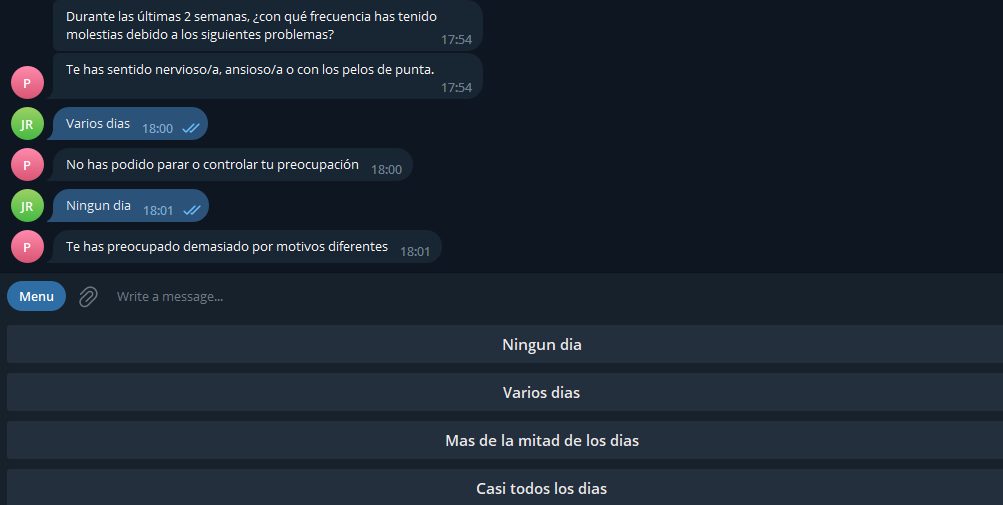
\includegraphics[width=0.8\textwidth, height=5.5cm]{imagenes/question.png}
    \caption{ Cuestionario de preguntas }
    \label{fig:cuestionario}
\end{figure}

Ya sabemos que cada pregunta cuenta con posibles respuestas de forma independiente. Cuando el bot hace la pregunta actualiza el teclado de Telegram y da la opción solo de contestar mediante botones que contienen las respuestas a la pregunta. Esto se hace de la siguente manera:

\begin{lstlisting}[language=Python]
#Function to get a custom keyboard in Telegram
def custom_keyboard(values):
    schema = [[str(value)] for value in values]
    return ReplyKeyboardMarkup(schema, one_time_keyboard=True, resize_keyboard=True)
\end{lstlisting}

El parámetro pasado contiene las respuestas a la pregunta y haciendo uso de la función \textit{ReplyKeyboardMarkup()} proporcionada por la libreria de Telegram creamos un teclado personalizado con los valores que deseemos. Solo se puede responder a la pregunta si el mensaje esta dentro de estas respuestas. Esto se ha hecho para asegurarse que los datos obtenidos son correctos y reales, ya que si se responde cualquier cosa que no tuviera nada que ver se guardaría como respuesta a la pregunta. Por lo que en cada iteracción de la función se comprueba si el mensaje proporcionado por el usuario es válido. En caso negativo, como se muestra en la \textit{\hyperref[fig:wrong]{Figura 5.22}} el bot no pasaría a la siguiente pregunta y volverá a realizarla de forma indefinida hasta que se responda de forma correcta. \vspace{0.5cm}

\begin{figure}[!ht]
    \centering
    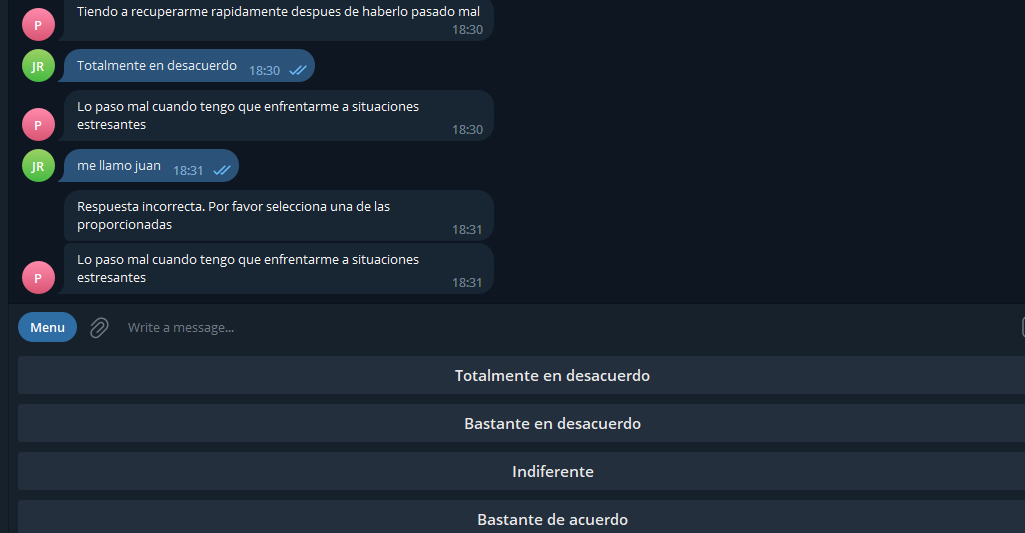
\includegraphics[width=1\textwidth]{imagenes/pregunta_incorrecta.png}
    \caption{ Mensaje del bot a una respuesta incorrecta }
    \label{fig:wrong}
\end{figure}\vspace{0.3cm}

Solo cuando esta sea correcta guardará la respuesta en la base de datos. La función finaliza cuando el usuario haya terminado de responder todas las preguntas y lo redirigirá de forma automática al módulo conversacional.

\begin{figure}[!ht]
    \centering
    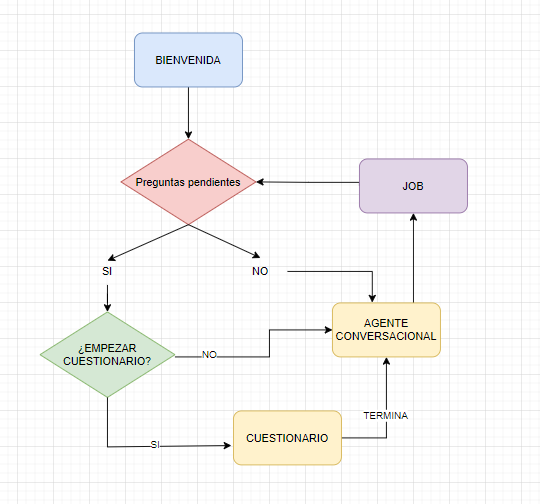
\includegraphics[width=0.8\textwidth, height=7.5cm]{imagenes/flujo.png}
    \caption{ Diagrama de flujo del bot}
    \label{fig:flujo}
\end{figure}
\vspace{1cm}

En la \textit{\hyperref[fig:flujo]{Figura 5.23}} se ve como sería el diagrama de flujo que sigue el bot y la lógica que utiliza. 

Recapitulando todo el proceso, cuando se inicie una conversación con el bot, este te registrará en la base de datos como un nuevo usuario. El sistema comprobará si hay algún cuestionario planificado para ese momento, en caso afirmativo el bot avisará al usuario y preguntará si desea realizar el cuestionario que se encuentre activo. Si se accede a responder, en el momento que termine se le llevará al módulo conversacional en el que puede charlar con el bot. Si no accede a responder, no pasaría nada, el cuestionario terminaría según lo planificado y no habría respuestas de el usuario para ese cuestionario. Una vez dentro de este módulo conversacional, el bot volverá a avisar a el usuario cuando haya de nuevo un cuestionario activo y continuaría con la misma dinámica.

\section{Tecnologías}
Para el desarrollo usaremos herramientas de Front-End, que nos ayudarán a dar cuerpo a nuestro sitio web y herramientas de Back-End para el control y lógica tanto de la web como del bot. Las tecnologías utilizadas para la implementación del proyecto son las siguientes:

\begin{itemize}
\item \textit{\textbf{Python}} como lenguaje principal del bot y de la web.
\item \textit{\textbf{Django}} es un framework de aplicaciones web gratuito y de código abierto (open source) escrito en Python para el desarrollo de nuestra web.
\item \textit{\textbf{Telegram}} como plataforma para alojar el chatbot
\item \textit{\textbf{Python-telegram-bot}} es una librería de Python para la creación de nuestro bot que nos permite conectarnos a la API de Telegram.
\item \textit{\textbf{PostgreSQL}} es un sistema de gestión de base de datos relacional orientado a objetos.
\item \textit{\textbf{Psycopg2}} para adaptar la base de datos a Python.
\item \textit{\textbf{HTML5}} lenguaje para la elaboración de páginas web.
\item \textit{\textbf{CSS3}} como lenguaje de diseño gráfico para crear la presentación de nuestra página.
\item \textit{\textbf{Javascript}} para dar dinamismo a nuestra web y ayudar en la experiencia del usuario.
\item \textit{\textbf{Foundation}} como framework de ayuda a la hora de crear la interfaz de usuario.
\item \textit{\textbf{Docker}} para automatizar el despliegue de la aplicación dentro de un contenedor software.
\item \textit{\textbf{Github}} como tecnología que nos ayuda a realizar copias del proyecto y controlar versiones.
\end{itemize}
